\documentclass[11pt,a4paper]{article} 

\usepackage[dutch]{babel} %needs to specified for minutes package (else it will be in German)
\usepackage{a4wide}%For a wider spacing of the text (smaller left/right margin)

\usepackage{setspace}
\usepackage{minutes}
\usepackage{graphicx}
\pagestyle{plain}
\usepackage{todositemized}
%more memmorable commands to make the checked and crossed symbols





%%%%%%%%%%%%%%%%%%%%%%%%%%%%%%%%%%%%%%%%%%%%%%%%%%%%%%%%%%%%%%%%%%%%%%%%%%%%%%%
%
% Important: This template compiles without errors
% always check errors, also the yellow ones, even if you get a PDF
%
%%%%%%%%%%%%%%%%%%%%%%%%%%%%%%%%%%%%%%%%%%%%%%%%%%%%%%%%%%%%%%%%%%%%%%%%%%%%%%%%





\newpage



\usepackage[dutch]{babel} %needs to specified for minutes package (else it will be in German)
\usepackage{a4wide}%For a wider spacing of the text (smaller left/right margin)

\usepackage{setspace}
\usepackage{minutes}

\pagestyle{plain}
\usepackage{todositemized}
%more memmorable commands to make the checked and crossed symbols





%%%%%%%%%%%%%%%%%%%%%%%%%%%%%%%%%%%%%%%%%%%%%%%%%%%%%%%%%%%%%%%%%%%%%%%%%%%%%%%
%
% Important: This template compiles without errors
% always check errors, also the yellow ones, even if you get a PDF
%
%%%%%%%%%%%%%%%%%%%%%%%%%%%%%%%%%%%%%%%%%%%%%%%%%%%%%%%%%%%%%%%%%%%%%%%%%%%%%%%%



\begin{document}

\begin{Minutes}{Notulen Poject Natuurkunde, groepje 24}


%Add relevant date, time and location here
\minutesdate{03-06-2023} %Write the date of when you finish the minutes
\starttime{10:00}
\endtime{}
\location{D0.115}

%Add relevant names here
\participant{Talha, Tom, Noah, Madelief} 
\minutetaker{Tom, Talha, Madelief}

% \moderation{Niemand} 
%In case people are not present


\maketitle



\newpage



\section{Mededelingen} 
Vandaag is de dag begonnen met uitleg van Antione (supervisor), hieronder wat aantekeningen die door Talha zijn gemaakt:
hoeveel energie is verloren op impact, hertz theory purely elastic, dan zal het niet terug naar oude positie.
for $U(y)=U_0 \frac{y}{h}$ 
$\eta$ is viscosity 
solids need constant force for constant deformation, not like liquid therapy puty, (silly putty), has the property of spreading out, it flows, even thiugh it has a high viscosity like a honey,it bounces,on short time scale viscoelasticliquid, it behaves like a solid, 
elastic solid, $\frac{F}{m^2}=\sigma$,$\sigma$ = stress, G times gamma, area is the crossectional area, gamma is deformation, G is elastic modulus, sheer: parallel force, extension is from both sides, But for viscous liquid,stress gamma dot times nu. 

\section{Begin experiment}
We hebben geleerd hoe de opstelling werkt, de programma's die we moeten gebruiken voor de beeldanalyse. 
Talha, Madelief en Noah hebben de opstelling veranderd zodat het wat praktischer is, we hebben twee stangen verbonden zodat we het balletje van boven kunnen ophangen zodat het altijd op ongeveer dezelfde plek valt. We hebben spuit met duct tape verbonden aan de stang, waaraan vervolgens weer een naald is verbonden waar de putty ingestoken kan worden. Deze valt dan langzaam omlaag totdat die loskomt en valt.
Terwijl deze opstelling werd gemaakt is Tom bezig geweest om een code te schrijven die het contactoppervlak kan bepalen van de bal op ieder moment van de vervorming.

\section{Overige punten}
n.v.t

\section{Figuren}
\begin{figure}[h]
    \centering
    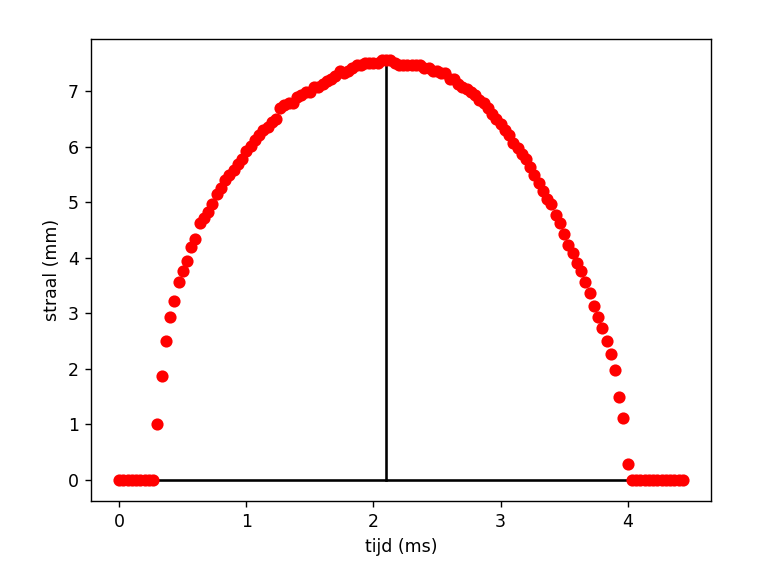
\includegraphics[width=0.5\linewidth]{straalbepalen.png}
    \caption{Voorbeeld van de data voor het bepalen van de straal}
    \label{fig:straalbepalen}
\end{figure}

\end{Minutes}
\end{document}


\section{Oude actiepunten}
Zijn er niet.

\section{Wat moeten we nu doen/bespreken?}

\subsection{Wie wil en kan wat?}

\task{talha}{checklist}

\subsection{Communicatie}


\subsection{Beschikbaarheid}


\section{Checklist uit de Powerpoint}



\section{Overige punten}
We wachten even morgen af, als we met Antoine spreken.

\section{Nieuwe actiepunten}
\listoftasks
\section{Volgende vergadering}
De volgende bijeenkomst is morgen met de begeleider, bij het fancy koffiezet apparaat bij D.

\section{Afsluiting vergadering}
De vergadering is om 12:49 gesloten.


\end{Minutes}
\end{document}